\chapter{RDMA 通信栈的设计与实现}\label{chap:RJIAJIA}{
本章主要介绍 M-JIAJIA系统中 RDMA 通信栈的架构设计与实现方案。作为通信层组件,RDMA 通信栈与 UDP 通信栈均可用于完成系统消息通信任务,用户可根据底层通信环境在系统运行前通过 .jiaconf 配置实现通信栈的动态切换。在架构设计上,RDMA 和 UDP 通信栈均采用多线程设计,但由于 RDMA通信栈与底层网络适配器深度集成,在实现上与 UDP 通信栈呈现显著差异。

RDMA 通信首先需要根据应用场景选择合适的通信模式和通信原语,并基于所选模式和原语构建 RDMA 通信管理器,以管理所需的通信资源。随后,根据通信链路模式执行建连后通信或无连接通信。

\section{设计概览}

\subsection{RDMA 通信模式与通信原语选择}
RDMA 支持四种通信模式:可靠连接(RC)、不可靠连接(UC)、可靠数据报(RD)、不可靠数据包(UD)。通信模式不仅决定数据传输的可靠性、有序性和连接方式,还影响通信原语的选择。不同的通信模式适用于不同的应用场景。

\textbf{RC 模式}: RC 模式采用面向连接的方式,提供可靠且有序的传输服务。通信开始前,需要在通信双方的RC QPs之间建立私有连接。连接建立后,双方将以消息为基本单元进行通信。

RC 模式具有可靠且有序的传输特性,且支持单向 Verbs 和原子操作,使其被广泛应用在对数据一致性、完整性和顺序性要求较高的场景中。例如,分布式存储系统 ~\citep{christopher2013pilaf, drago2014farm, xingda2020xstore}、高性能计算 ~\citep{graham2005OpenMPI, Huang2006MVAPICH2} 以及分布式事务系统 ~\citep{xingda2018DrTM+H} 等领域。

\textbf{UC 模式}:UC 模式可视为 RC 模式的子集,面向连接但提供不可靠的传输服务(即不提供 Ack/Nak响应机制,不保证消息被对端成功接收),
适用于对可靠性要求较低但对性能要求较高的场景,例如某些对实时性要求较高的视频应用。
此外,在具备强大容错机制的分布式系统中 ~\citep{kalia2014herd},UC 模式相比于 RC 模式可减少网络间通信流量,提升数据传输效率。

\textbf{RD 模式}:目前尚未有硬件支持 RD 模式,因此该模式尚未在实际应用中得到推广。

\textbf{UD 模式}:UD 模式提供不可靠的数据报服务,无需建立连接,单个 QP 即可通过单播、多播或广播与其他 UD QPs 进行通信,但最大消息大小受 MTU 限制,适用于对可靠性要求较低或在应用层实现可靠性、规模较大且需要多播的应用场景~\citep{kalia2014herd,kalia2016fasst}。

M-JIAJIA 在可靠连接(RC)模式下采用 Send 原语进行消息传递,这一设计选择主要基于考虑 
M-JIAJIA 对通信可靠性要求严格,而 RC 模式不仅免除了应用层的分片处理,还省去了额外的可靠性与有序性保障,从而大大简化了系统设计。

图~\ref{fig:mjiajia-send-recv}显示了 RC 模式下使用 Send 原语发送固定大小消息的示例,图中省略了队列对之间的私有连接以及完成队列元素的生成与处理。为了实现图示通信,M-JIAJIA 采用 RDMA CM 完成建连操作。而且考虑到发送与接收的差异,M-JIAJIA 使用公共输出队列与连接私有输入队列的方案来降低消息队列空间占用。此外,M-JIAJIA 应用多线程优化通信架构设计,以提升整体性能。
\begin{figure}[H]
    \centering
    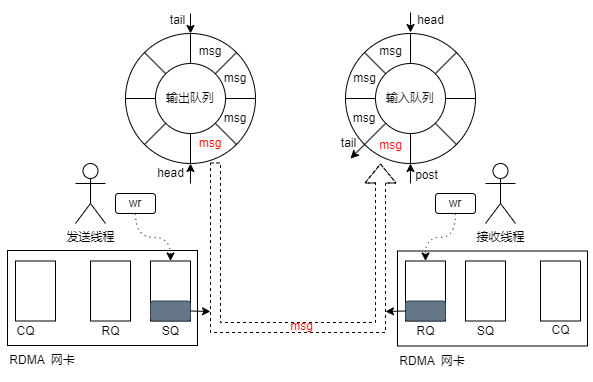
\includegraphics[width=\textwidth]{Img/RDMA-send-receive.png}
    \bicaption{\enspace RDMA 通信栈可靠连接 Send 示例}{\enspace RDMA communication stack reliable connection Send example}
    \label{fig:mjiajia-send-recv}
\end{figure}



\subsection{RDMA 通信管理器设计}

M-JIAJIA 的 RDMA 通信管理器(jia\_context\_t)旨在管理 RDMA 通信所涉及的资源和配置参数。具体可分为以下几部分:

\begin{enumerate}[label=\arabic*., leftmargin=1em, align=left]
    \item \textbf{RDMA 设备相关信息}
        \begin{itemize}
            \item \textbf{设备上下文}:设备上下文是应用程序与 RDMA 硬件之间的接口,用于管理所有其他 RDMA 资源。
            \item \textbf{设备端口号}:设备端口号用于标识 RDMA 设备进行通信的物理端口。
        \end{itemize}

    \item \textbf{RDMA 资源管理信息}
        \begin{itemize}
            \item \textbf{保护域}:保护域(Protect Domain, PD)是一种资源隔离手段,在RC 模式下用于限制 QPs 可以访问内存区域(Memory Region,MR)的范围。
            \item \textbf{内存区域}:内存区域是应用程序注册后可被 RDMA 设备直接访问的内存。M-JIAJIA 采用 Send 原语进行通信,因此需分别为发送和接收准备独立的内存区域。在多通信场景下,考虑到输入的不确定性,M-JIAJIA 采用单输出、多输入的内存区域设计方案。
        \end{itemize}

    \item \textbf{RDMA 事件通知信息}
        \begin{itemize}
            \item \textbf{完成事件通道}:完成事件通道提供 CQ 事件通知机制,用于通知工作请求是否完成。M-JIAJIA 提供独立的发送和接收完成事件通道。
        \end{itemize}

    \item \textbf{RDMA 连接管理信息}
        \begin{itemize}
            \item \textbf{RDMA 连接管理结构}:该结构用于管理与每个连接相关的信息。包括连接状态、发送序号和接收序号、RDMA 连接管理标识符(rdma\_cm\_id)、输入队列和输入内存区域。
            \item \textbf{RDMA 连接管理结构数组}:连接管理结构数组记录了与每个远端节点的连接信息。
            \item \textbf{RDMA 建立连接线程标识}:M-JIAJIA 采用客户端-服务器模式建立连接。在建连阶段,节点分别创建客户端和服务器线程以完成连接。其建连方案具有独特性:每个节点至多创建一个服务器线程用于监听连接请求,同时可创建多个客户端线程主动发起连接。线程标识用于存储和管理线程的信息,便于线程创建、同步和管理。
        \end{itemize}
        
    \item \textbf{配置参数}
        \begin{itemize}[leftmargin=*, nosep]
            \item \textbf{批处理数目}: 该参数在 M-JIAJIA 中用于指定在下发接收工作请求时一次下发的工作请求的数量
        \end{itemize}
\end{enumerate}

% \begin{lstlisting}[style=CStyle]
% typedef struct jia_context {
%     struct ibv_context *context;
%     struct ibv_pd *pd;                      // common pd
%     struct ibv_comp_channel *recv_comp_channel;  // common recv io completion channel
%     struct ibv_comp_channel *send_comp_channel;

%     // port related
%     int ib_port;                   // ib port number

%     // info data
%     int batching_num; // post recv wr doorbell batching num

%     // rdma connect (Maxhosts inqueues, only one outqueue)
%     msg_queue_t *outqueue;
%     struct ibv_mr *out_mr[QueueSize];
%     rdma_connect_t connect_array[Maxhosts];

%     // connection parameters
%     pthread_t server_thread;   // server thread for connection from client on other hosts
%     pthread_t *client_threads; // client threads used to connect other hosts
% } jia_context_t;

% typedef struct rdma_connect {
%     bool connected;
%     unsigned    snd_seq;
%     unsigned    rcv_seq;
%     struct rdma_cm_id id;

%     struct ibv_mr **in_mr;
%     msg_queue_t *inqueue;
% } rdma_connect_t;
% \end{lstlisting}

\subsection{RDMA 通信栈组成模块}

为构建基于 RDMA 可靠连接(RC)的通信系统,RDMA 通信栈的初始化流程分为以下四个主要阶段(如图~\ref{fig:mjiajia-rdma-modules}右侧所示):
\begin{enumerate}[label=\arabic*.]
    \item 初始化上下文。包括获取设备列表、选择硬件设备、打开设备获取上下文、配置物理端口以及输入/输出消息队列初始化等步骤。
    \item 建立连接。通过创建线程向其他主机发起建连请求、并响应其他主机的连接请求,完成任意两节点之间的建连。
    \item 初始化通信资源。主要用于注册输入/输出内存区域(MR)。
    \item 多线程通信。创建线程分别负责下发发送/接收工作请求(WR),同时创建专门处理消息的线程,以优化通信效率。
\end{enumerate}

\begin{figure}[!htbp]
    \centering
    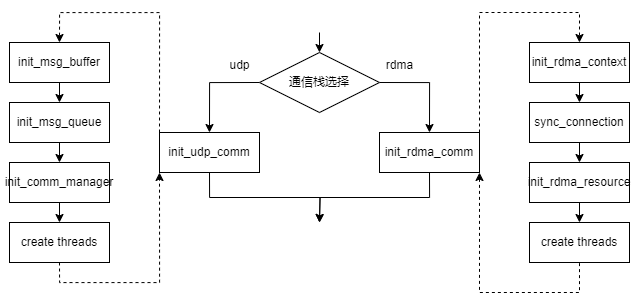
\includegraphics[width=\textwidth]{Img/RDMA-comm-modules.png}
    \bicaption{\enspace M-JIAJIA 通信栈}{\enspace M-JIAJIA communication stack}
    \label{fig:mjiajia-rdma-modules}
\end{figure}

\section{可靠通信连接建立机制}
M-JIAJIA 采用基于 RDMA CM 的建连方式。该方式具有三个显著优势:
\begin{enumerate}[label=\arabic*.]
    \item 编程简单,RDMA CM 封装了底层复杂的连接建立过程,(使开发者无需直接操作Verbs API即可完成通信流程。
    \item 开销低,RDMA CM 支持异步操作模式,通过事件通道(Event Channel)实现非阻塞通信,避免轮询带来的开销。
    \item 可移植性强,RDMA CM 兼容InfiniBand、RoCEV2和iWARP多种 RDMA 实现,无需针对不同硬件进行代码修改。
\end{enumerate}

如图~\ref{fig:mjiajia-cm-connection}所示,建连过程需要客户端和服务器紧密配合,共同完成一系列复杂的步骤,最终生成用于通信的 rdma\_cm\_id 。

\begin{figure}[H]
    \centering
    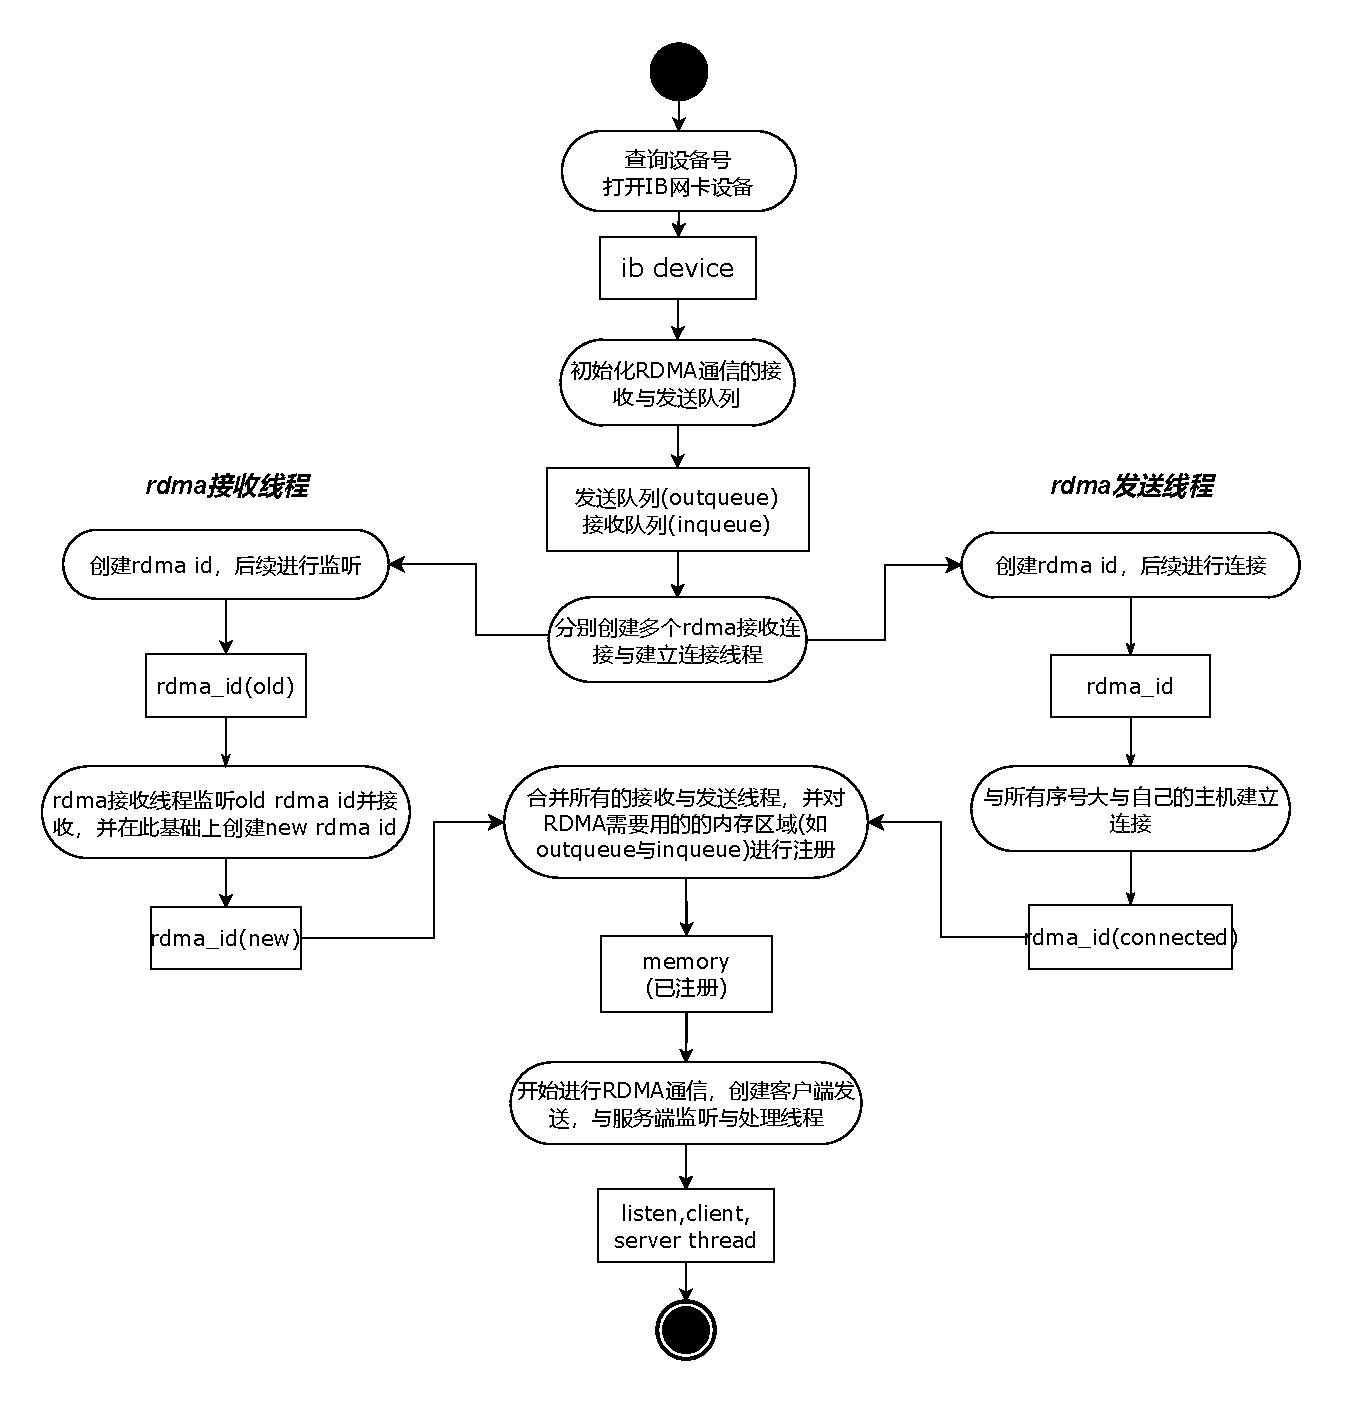
\includegraphics[width=\textwidth]{Img/rdma_init.drawio.pdf}
    \bicaption{M-JIAJIA RDMA CM 建连流程图}{M-JIAJIA RDMA CM Connection Establishment Flowchart}
    \label{fig:mjiajia-cm-connection}
\end{figure}

\subsection{建连客户端与服务器}

% \begin{algorithm}
%     \caption{RDMA Client Connection Thread}
%     \begin{algorithmic}[1]
%         \Procedure{SyncClientThread}{arg}
%             \State $server\_id \gets$ \Call{ConvertToInt}{arg}
%             \State $retry\_flag \gets true$, $retry\_count \gets 0$

%             \State $ec \gets$ \Call{RdmaCreateEventChannel}{}

%             \While{$retry\_flag$ \textbf{and} $retry\_count < MAX\_RETRY$}
%                 \State $retry\_flag \gets false$
%                 \State $id \gets$ \Call{RdmaCreateId}{$ec$}
%                 \State $addr \gets$ \Call{SetAddress}{$server\_id$}
%                 \State \Call{RdmaResolveAddr}{$id$, $addr$, $2000$}

%                 \State
%                 \While{true}
%                     \State \Call{RdmaGetCmEvent}{$ec$, $event$}

%                     \If{$event.type = RDMA\_ROUTE\_RESOLVED$}
%                         \State $client\_id \gets event.param.conn.private\_data$
%                         \State $ctx.recv\_comp\_channel \gets$ \Call{CreateCompletionChannel}{}
%                         \State $ctx.send\_comp\_channel \gets$ \Call{CreateCompletionChannel}{}

%                         \State
%                         \State Initialize $qp\_attr$
%                         \State Request CQ notifications
%                         \State $ctx.pd \gets$ \Call{Allocate}{$event.id$}
%                         \State \Call{CreateQP}{$event.id$, $ctx.pd$, $qp\_attr$}

%                         \State
%                         \State Initialize $conn\_param$
%                         \State $event.id \gets$ \Call{RDMAConnect}{$conn\_param$}
%                     \ElsIf{$event.type = RDMA\_ESTABLISHED$}
%                         \State Update $ctx.connect\_ array[client\_id]$ connection status
%                     \Else
%                         \State \textbf{Default action}
%                     \EndIf

%                     \State \Call{RdmaAckCmEvent}{$event$}
%                 \EndWhile

%                 \Statex \textbf{NextTry:}
%             \EndWhile

%             \Statex \textbf{Cleanup:}
%             \State \Call{RdmaDestroyEventChannel}{$ec$}
%             \State \Return NULL
%         \EndProcedure
%     \end{algorithmic}
% \end{algorithm}

% \begin{algorithm}
% \caption{RDMA Synchronization Server Thread}
% \begin{algorithmic}[1]
%     \State $ec \gets$ \Call{Create\_event\_channel}{$ $} \;
%     \State $listener \gets$ \Call{Create\_RDMA\_listener\_ID}{$ $} \;
%     \State Initialize $addr \gets \{ip, start\_port + jia\_pid\}$ \;
%     \State \Call{Bind\_addr}{$listener, addr$} \;
%     \While{true}
%         \State $event \gets$ \Call{rdma\_get\_cm\_event}{$ec$} \;
%         \If{$event.type = $RDMA\_CM\_EVENT\_CONNECT\_REQUEST}
%             \State $client\_id \gets event.param.conn.private\_data$ \;
%             \State $ctx.recv\_comp\_channel,ctx.send\_comp\_channel \gets$ \Call{create\_completion\_channel}{$ $} \;

%             \State
%             \State Initialize $qp\_attr$ \;
%             \State Request CQ notifications \;
%             \State $ctx.pd \gets$ \Call{allocate}{$event.id$} \;
%             \State \Call{create\_QP}{$event.id$, $ctx.pd$, $qp\_attr$} \;

%             \State
%             \State Initialize $conn\_param$ \;
%             \State $event.id \gets$ \Call{RDMA\_accept}{$conn\_param$} \;
%         \ElsIf{$event.type = $RDMA\_CM\_EVENT\_ESTABLISHED}
%             \State Update $ctx.connect\_array[client\_id]$ connection status \;
%             \State $completion\_num \gets completion\_num + 1$ \;
%             \If{$completion\_num = system\_setting.jia\_pid$}
%                 \State \textbf{goto} Cleanup \;
%             \EndIf
%         \Else \quad \textbf{Default action} \;
%         \EndIf
%         \State \Call{rdma\_ack\_event}{$event$} \;
%     \EndWhile

%     \State
%     \State \textbf{Cleanup:} \;
%     \State \Call{Destroy\_RDMA\_listener\_ID}{$listener$} \;
%     \State \Call{Destroy\_event\_channel}{$ec$} \;
%     \State \Return \;
% \end{algorithmic}
% \end{algorithm}

\subsection{RDMA 集群建连算法}

M-JIAJIA 运行时要求任意两节点具备通信能力,因此必须在任意两节点之间至少建立一个连接。
M-JIAJIA 采用客户端服务器模式,通过创建多个客户线程与服务线程去建立连接,并采用了算法~\ref{alg:connection-algo}所示的建连算法,
不必为每个连接设立单独的服务器处理。

\begin{algorithm}
\caption{RDMA Cluster Connection Establishment Algorithm}\label{alg:connection-algo}
\begin{algorithmic}[1]
\Procedure{sync\_connection}{$hosts$, $pid$}
\If{$pid$ $\neq$ 0}
\State \Call{pthread\_create}{\&ctx.server\_thread, NULL, server\_thread, \&ctx}
\EndIf
\State $num\_clients$ $\gets$ $hosts$ - $pid$ - 1
\If{$num\_clients$ $>$ 0}
\State $ctx.client\_threads$ $\gets$ \Call{malloc}{$num\_clients$ * sizeof(pthread\_t)} 
\For{$i \gets 0$ to $num\_clients$}
\State $target\_hosts$ $\gets$ \Call{malloc}{sizeof(int)}
\State $*target\_hosts$ $\gets$ $pid + i + 1$
\State \Call{pthread\_create}{\&ctx.client\_threads[i], NULL, client\_thread, target\_hosts}
\EndFor
\EndIf
\If{$pid$ $\neq$ 0}
\State \Call{pthread\_join}{ctx.server\_thread, NULL}
\EndIf

\If{$num\_clients$ > 0}
\For{$i \gets 0$ to $num\_clients$}
\State \Call{pthread\_join}{ctx.client\_threads[i], NULL}
\EndFor
\EndIf
\EndProcedure
\end{algorithmic}
\end{algorithm}

在rdma同步的过程中,主机号偏小的主机会创建多个client线程与主机号偏大的主机server线程尝试建立连接;
同时除jia\_pid为0外所有的主机都会创建一个server线程来监听建立的rdma连接,最终每两台主机之间建立一个rdma连接;
如图~\ref{fig:RDMA-connection-build}所示,创建线程并建立连接。



\begin{figure}[H]
    \centering    
    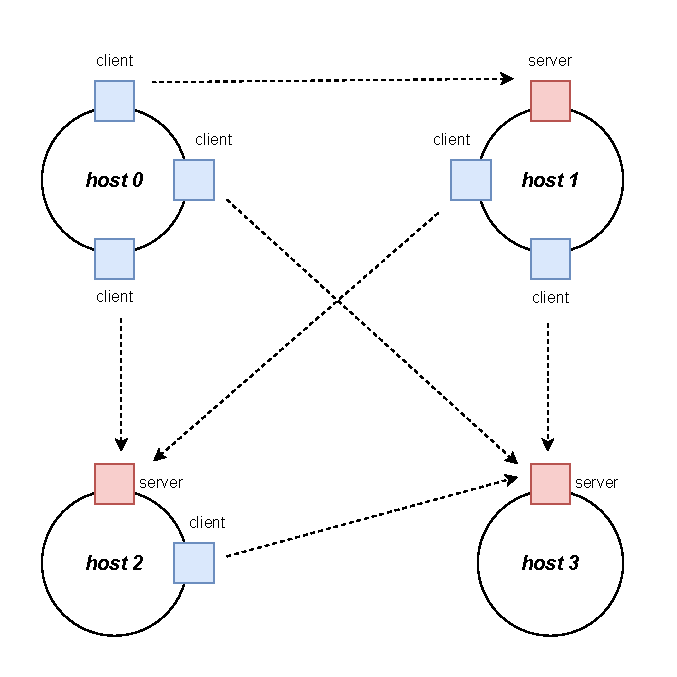
\includegraphics[width=0.65\textwidth]{Img/rdma_sync.drawio.pdf}
    \bicaption{\enspace RDMA集群建连示例}{\enspace RDMA Cluster Connection Establishment Example}
    \label{fig:RDMA-connection-build}
\end{figure}



% \begin{figure}[H]
%     \centering
% .    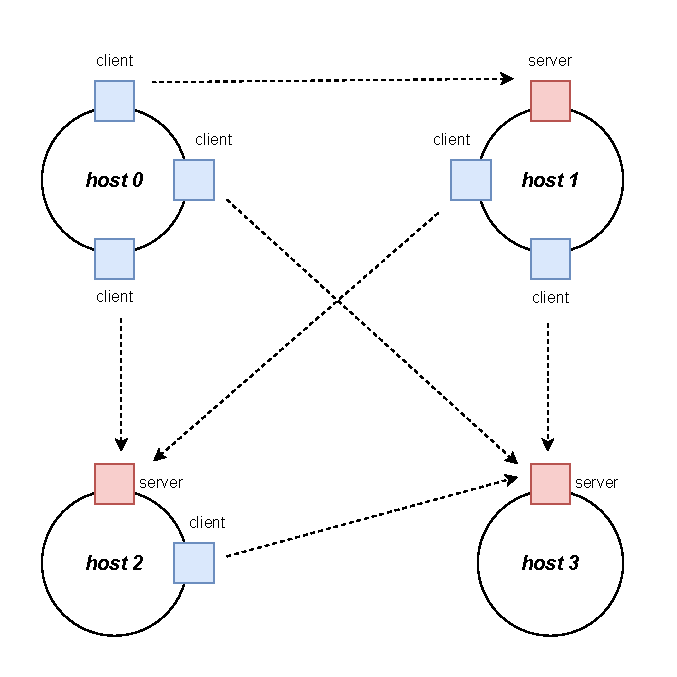
\includegraphics[width=1.0\textwidth]{Img/rdma_sync.drawio.pdf}
%     \caption{RDMA同步过程中的client与server同步线程}
% \end{figure}



\section{RDMA 多线程通信架构设计}

\begin{figure}[H]
    \centering
    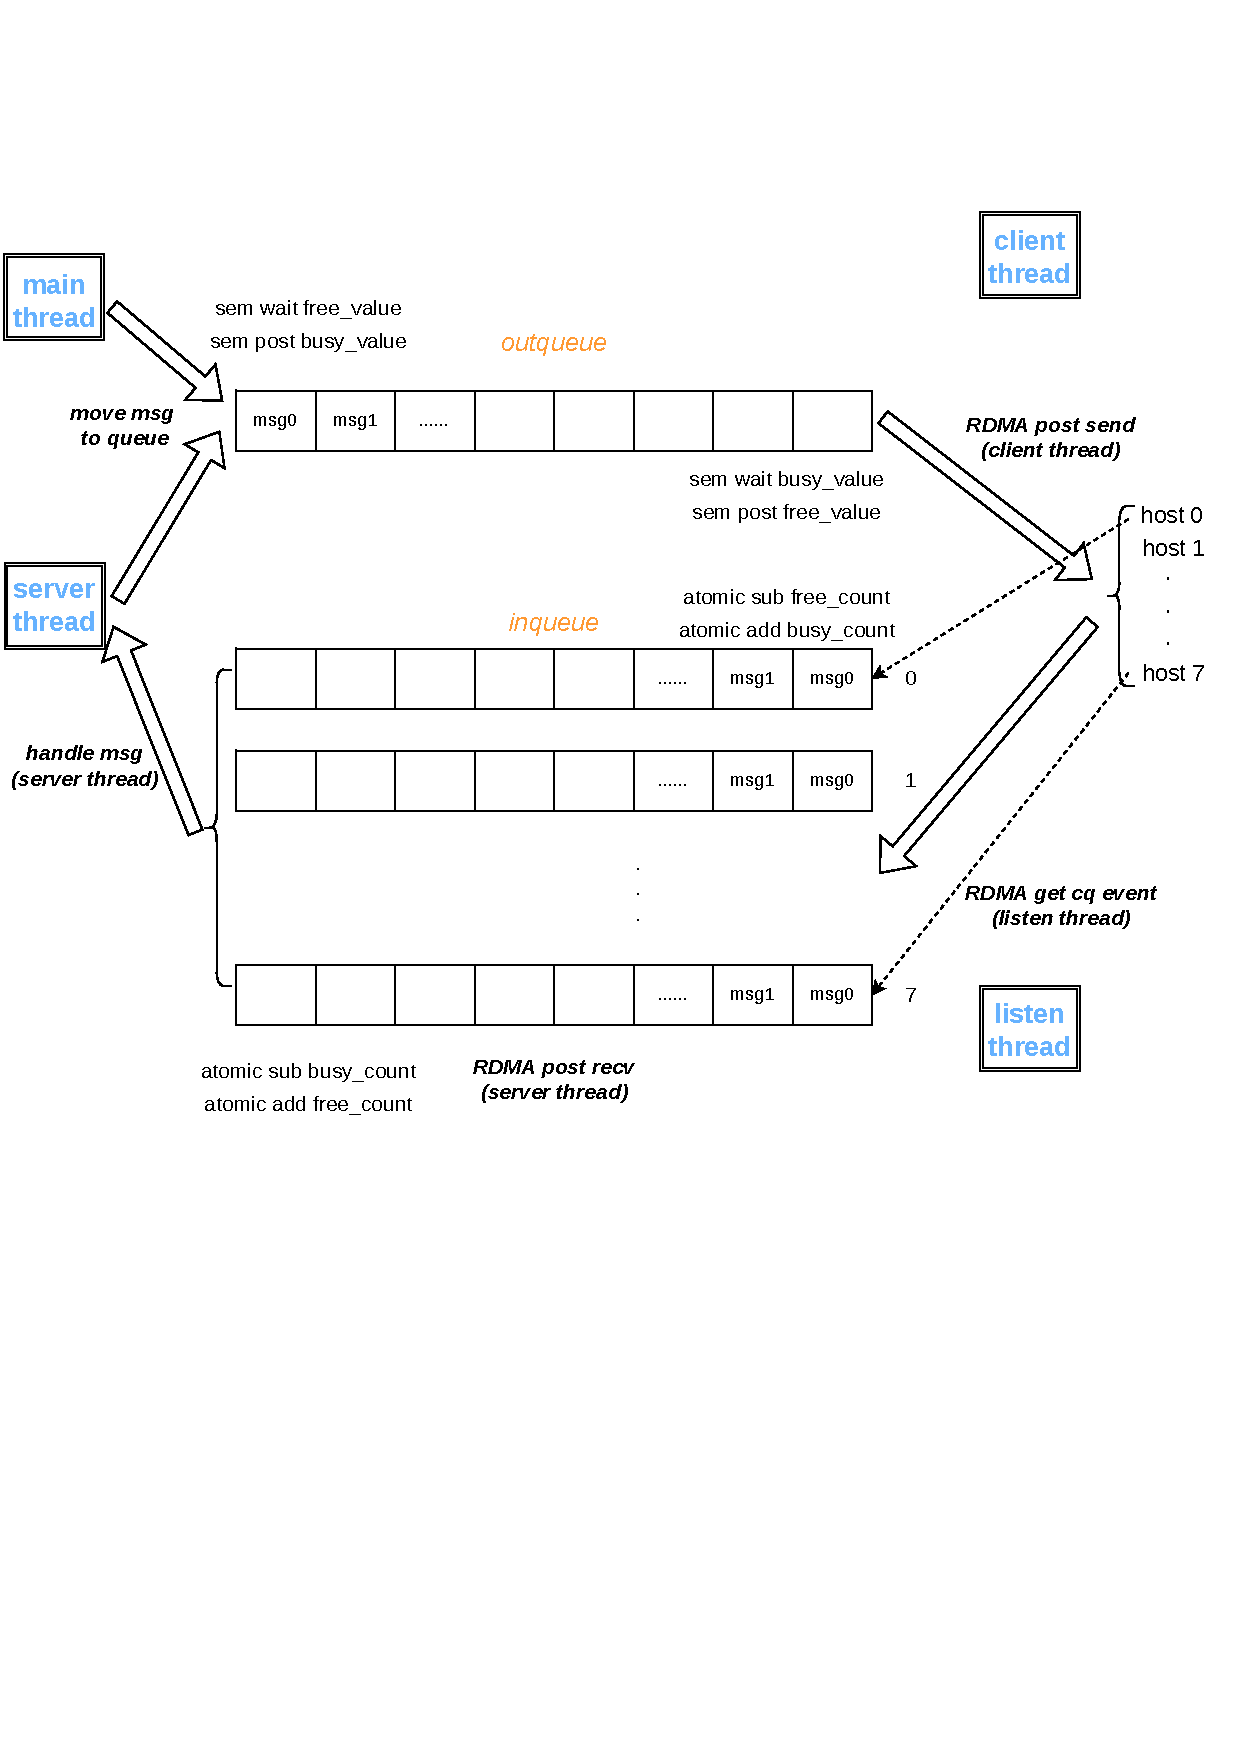
\includegraphics[width=1.1\textwidth]{Img/RDMA_design.pdf}
    \caption{RDMA communication design}
\end{figure}


\subsection{RDMA 多线程任务划分}

\subsubsection{RDMA通信接收端线程任务划分}
RDMA通信接收端由listen与server两个线程组成,他们的任务划分如下:

\begin{itemize}[leftmargin=*, nosep]
    \item \textbf{listen thread}:用于监听rdma接收到的msg,并通知server线程进行处理;
    \item \textbf{server thread}:用于处理rdma接收到的msg,同时负责下发任务,即在成功处理完成一个msg后post\_recv该空位,用于下一次接收;
\end{itemize}

\begin{figure}[H]
    \centering
.    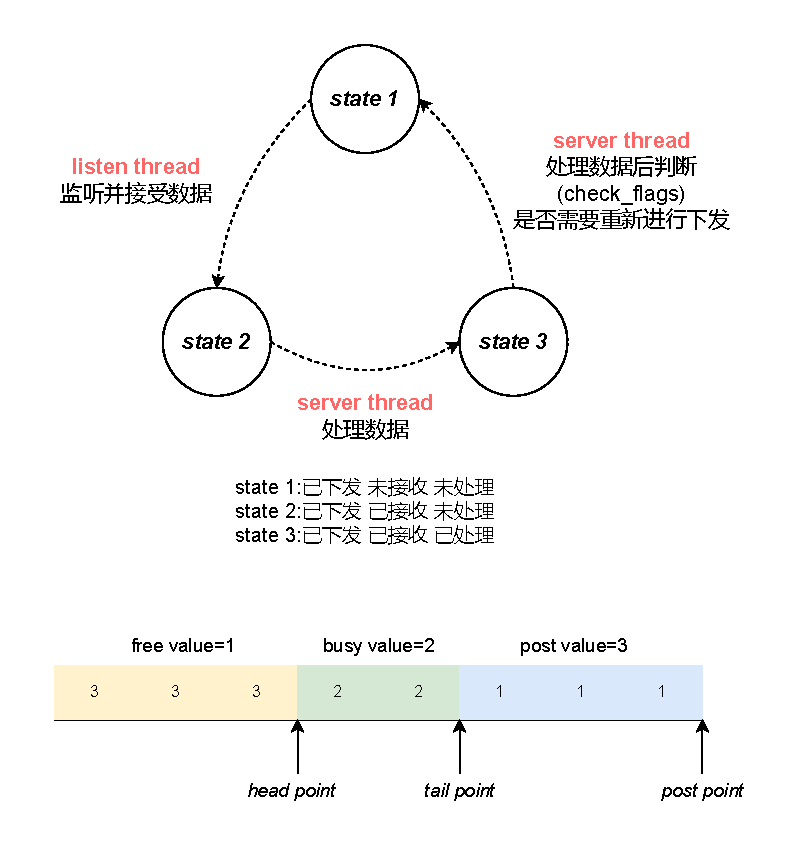
\includegraphics[width=1.0\textwidth]{Img/recv_state.drawio.pdf}
    \caption{RDMA接收端inqueue中msg的状态转换}
\end{figure}
        
listen thread的伪代码如下:
\begin{algorithm}
    \caption{listen thread algorithm}
    \begin{algorithmic}[1] % [1] 使得每行都有行        
        \Procedure{ListenThread}{}
            \State \Call{post\_recv}{$ $}
            \State \textbf{return} NULL
        \EndProcedure

        \Function{post\_recv}{}
            \While{$true$}
                \State $\{ cq\_ptr, context\} \gets$ \Call{ibv\_get\_cq\_event}{$recv\_comp\_channel$} 
                \State $inqueue \gets (rdma\_connect\_t)context.inqueue$
                \State \Call{ibv\_req\_notify\_cq}{$cq\_ptr$}
                \State $wc \gets$ \Call{ibv\_poll\_cq}{$cq\_ptr$}

                \State
                \If{$wc.status \neq \text{IBV\_WC\_SUCCESS}$}
                    \State \Call{log\_err}{$post\_recv \quad error$}
                \Else
                    \State \Call{atomic\_fetch\_sub}{$inqueue$->$post\_value$} 
                    \State \Call{atomic\_fetch\_add}{$inqueue$->$busy\_value$}

                    \State
                    \State $connect\_array[inqueue$->$queue[inqueue$->$tail]$->$topid].rcv\_seq $++
                    \State $inqueue$->$tail \gets (inqueue$->$tail$+1$) \% QueueSize$
                \EndIf
            \EndWhile
            
            \State
            \State \Call{ibv\_ack\_cq\_events}{$cq\_ptr$}
            \State \textbf{return}
        \EndFunction
    \end{algorithmic}
\end{algorithm}

\newpage
server thread的伪代码如下:
\begin{algorithm}
    \caption{server thread algorithm}
    \begin{algorithmic}[1] % [1] 使得每行都有行号
        \Procedure{ServerThread}{}
            \State \Call{init\_post\_recv\_wr}{$ $}

            \While{$true$}
                \For{$i \gets 0$ to $hostc$}
                    \State $tmp\_connect \gets connect\_array[i]$
                    \State $in\_queue \gets tmp\_connect$->$inqueue$
                    \If{\Call{atomic\_load}{$tmp\_connect.inqueue$->$busy\_value$}}
                        \State \Call{msg\_handle}{$inqueue$->$queue[head]$}
                        \State \Call{atomic\_fetch\_sub}{$inqueue$->$busy\_value$} 
                        \State \Call{atomic\_fetch\_add}{$inqueue$->$free\_value$}
                        \If{$i == jia\_pid$}
                            \State $tmp\_connect.rcv\_seq$ ++
                        \EndIf
                        \State $inqueue$->$head \gets (inqueue$->$head$+1$) \% QueueSize$
                    \EndIf
                \EndFor

                \If{$i \neq jia\_pid$}
                    \State \Call{check\_flags}{$i$}
                \EndIf
            \EndWhile
            \State \textbf{return}
         \EndProcedure
    \end{algorithmic}
\end{algorithm}

\newpage
\subsubsection{RDMA通信发送端线程任务划分}
RDMA通信接收端由main/server两个入队线程,和一个client发送线程组成,他们的任务划分如下:

\begin{itemize}[leftmargin=*, nosep]
    \item \textbf{main/server thread}:用于下发rdma需要发送的msg,并将msg放入outqueue队列中;
    \item \textbf{client thread}:将对应的msg从outqueue队列中取出,并通过rdma发送msg给对应主机;
\end{itemize}

client thread的伪代码如下:
\begin{algorithm}
    \caption{client thread algorithm}
    \begin{algorithmic}[1] % [1] 使得每行都有行号
        \Procedure{ClientThread}{}
            \While{$true$}
                \State \Call{sem\_wait}{$outqueue.busy\_count$}
                \State $msg\_ptr \gets$ \Call{dequeue}{$outqueue$}
                \State $msg\_ptr$->$seqno \gets connect\_array[msg\_ptr$->$to\_pid]$

                \State
                \If{$msg\_ptr$->$topid$ = $jia\_pid$}
                    \State \Call{memcpy}{$inqueue[tail],msg\_ptr$} 
                    \State \Call{atomic\_fetch\_sub}{$inqueue$->$free\_value$} 
                    \State \Call{atomic\_fetch\_add}{$inqueue$->$busy\_value$}
                    \State $inqueue$->$tail \gets (inqueue$->$tail$+1$) \%QueueSize$
                \Else
                    \While{\Call{post\_send}{$connect\_array[msg\_ptr$->$to\_pid]$}}
                    \EndWhile
                \EndIf
                
                \State
                \State $connect\_array[msg\_ptr$->$topid].snd\_seq$++
                \State $inqueue$->$head \gets (inqueue$->$head$+1$) \% QueueSize$
                \State \Call{sem\_post}{$outqueue.free\_count$}
            \EndWhile
            \State \textbf{return}
        \EndProcedure
    \end{algorithmic}
\end{algorithm}


\begin{algorithm}
    \caption{client thread post send}
    \begin{algorithmic}[1] % [1] 使得每行都有行号
        \Function{post\_send}{}
            \State initialize $sge \gets \{out\_mr[outqueue$->$head] \}$
            \State initialize $wr \gets \{sge\}$ 

            \State
            \State $msg\_ptr \gets$ $outqueue[outqueue$->$head]$

            \While{\Call{ibv\_post\_send}{$connect\_array[msg\_ptr$->$pid]$}}
            \EndWhile

            \State
            \State $cq\_ptr \gets$ \Call{ibv\_get\_cq\_event}{$send\_comp\_channel$}
            \State \Call{ibv\_req\_notify\_cq}{$cq\_ptr$}

            \State
            \State $wc \gets$ \Call{ibv\_poll\_cq}{$connect\_array[msg\_ptr$->$topid]$->$send\_cq$}
            \If{$wc.status \neq \text{IBV\_WC\_SUCCESS}$}
                \State \textbf{return} $1$
            \EndIf

            \State
            \State \Call{ibv\_ack\_cq\_events}{$cq\_ptr$}
            \State \textbf{return} $0$
        \EndFunction
    \end{algorithmic}
\end{algorithm}

\begin{figure}[H]
    \centering
    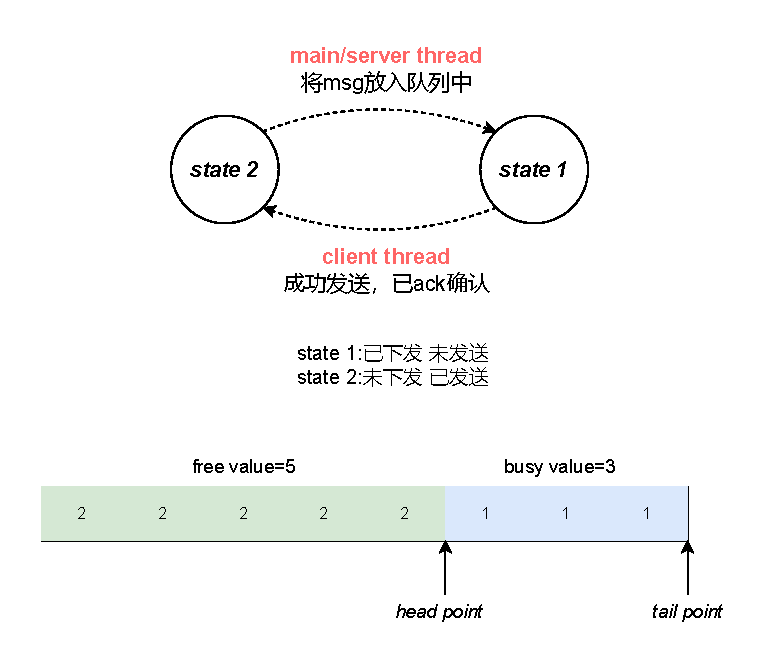
\includegraphics[width=1.0\textwidth]{Img/send_state.drawio.pdf}
    \caption{RDMA发送端outqueue中msg的状态转换}
\end{figure}


\newpage
\subsection{RDMA 多线程通信流程}

\subsubsection{消息发送流程}
\begin{enumerate}[leftmargin=1em, align=left]
    \item \textbf{消息入队}:
        \begin{itemize}[leftmargin=*, nosep]
            \item 应用程序将待发送的消息放入\texttt{outqueue}队列中,队列中的每个消息包含目标主机的IP地址和消息内容。
        \end{itemize}
    \item \textbf{RDMA Send操作}:
        \begin{itemize}[leftmargin=*, nosep]
            \item 发送端根据消息中的目标主机IP地址,查找对应的RDMA连接上下文(包括QP(Queue Pair)和MR(Memory Region)等信息)。
            \item 调用\texttt{ibv\_post\_send} API,将消息内容通过RDMA Send操作发送到目标主机。
        \end{itemize}
    \item \textbf{发送完成检测}: 
        \begin{itemize}[leftmargin=*, nosep]
            \item 发送端通过轮询或事件通知机制(如Completion Queue)检测Send操作的完成状态。
            \item 当检测到Send操作成功完成时,发送端从\texttt{outqueue}队列中移除已发送的消息,并准备发送下一条消息。
        \end{itemize}
    \item \textbf{错误处理}: 
        \begin{itemize}[leftmargin=*, nosep]
            \item 如果Send操作失败,发送端会记录错误日志,并根据配置决定是否重试发送或丢弃该消息。
        \end{itemize}
\end{enumerate}

\subsubsection{消息接收流程}
\begin{enumerate}[leftmargin=1em, align=left]
    \item \textbf{预置Recv Buffer}:
        \begin{itemize}[leftmargin=*, nosep]
            \item 接收端在初始化时,预先为每个QP下发多个Recv Buffer,通过\texttt{ibv\_post\_recv} API将Recv请求提交到接收队列中。
            \item 每个Recv Buffer对应一个内存区域,用于存储接收到的消息。
        \end{itemize}
    \item \textbf{消息接收}:
        \begin{itemize}[leftmargin=*, nosep]
            \item 当发送端发起RDMA Send操作时,接收端的RNIC(RDMA Network Interface Card)会将消息数据直接写入预置的Recv Buffer中。
            \item 接收端通过轮询或事件通知机制检测Recv操作的完成状态。
        \end{itemize}
    \item \textbf{消息入队}: 
        \begin{itemize}[leftmargin=*, nosep]
            \item 当检测到Recv操作完成时,接收端将接收到的消息从Recv Buffer中取出,并放入\texttt{inqueue}队列中。
            \item 接收端继续下发新的Recv请求,以确保始终有足够的Recv Buffer接收后续的消息。
        \end{itemize}
    \item \textbf{消息处理}: 
        \begin{itemize}[leftmargin=*, nosep]
            \item 接收端的服务线程(Server Thread)定期轮询\texttt{inqueue}队列,取出消息并进行处理。
            \item 处理逻辑由应用程序定义,可能包括数据解析、业务逻辑处理、响应生成等。
        \end{itemize}
\end{enumerate}


\section{本章小结}本章主要介绍了RDMA通信栈的设计与实现。首先简要介绍RDMA几种常见的通信模式,并探讨了在M-JIAJIA中RDMA的基本通信组成模块和流程;随后介绍了RDMA建连过程中每台主机的client线程与server线程的运作原理;最后探讨了在RDMA通信过程中每台主机相关线程的通信流程。

本章 4.1 节给出 M-JIAJIA RDMA通信模式与通信原语选择。首先介绍了RDMA基本的几种通信模式(RC,UC,RD,UD模式),并通过画图阐述了M-JIAJIA在RC模式下的通信基本流程;然后探讨了RDMA通信管理器中的相关信息以及通信栈组成模块,并通过画图揭示了RDMA通信的一般流程;

本章 3.2 节主要介绍 M-JIAJIA 的函数接口。首先,阐述了全局变量 jiahosts 和 jiapid 的作用;随后,详细解析了 jia\_init 初始化模块的执行流程,并介绍 M-JIAJIA 在该模块上的架构优化。接着,探讨了共享内存的分配算法及其对应的接口设计,进一步介绍了消息传递接口和 RMA 接口。最后,以模块概述和使用说明作为小节总结。

本章 3.3 节介绍了 M-JIAJIA 的核心模块设计,涵盖初始化模块、系统配置模块、内存管理模块、锁管理模块、UDP 通信管理模块、RDMA 通信管理模块及统计模块,并简要阐述其功能与实现机制。

本章 3.4 节介绍了 M-JIAJIA 的通信层设计,该层包括 UDP 通信栈和 RDMA 通信栈。本节重点探讨 UDP 通信栈的设计,首先阐述 M-JIAJIA 端口占用算法如何将端口占用的复杂度从 $O(n^2)$ 降至 $O(n)$。随后,对比 Linux 系统中的三种多路复用接口——select()、poll() 和 epoll(),并分析 M-JIAJIA 选择 epoll 的原因。接着,介绍 M-JIAJIA 多线程架构设计相较于 JIAJIA 信号驱动 I/O 的优势,并详细说明发送线程、侦听线程和服务线程的实现机制。最后,探讨 M-JIAJIA 如何通过序号、确认及超时重传机制实现可靠通信。

本章 3.5 节介绍了 M-JIAJIA 的远程预取优化机制,包括共享内存初始化过程中常见的两次消息传递获取写权限模式,以及针对与此 M-JIAJIA 的预取策略。

本章 3.6 节简要介绍了 M-JIAJIA 在提高系统易用性和可维护性上的工作。包含配置文件和日志机制两部分。
}